\documentclass[document.tex]{subfiles}
\begin{document}
\section*{Exercise 2:}


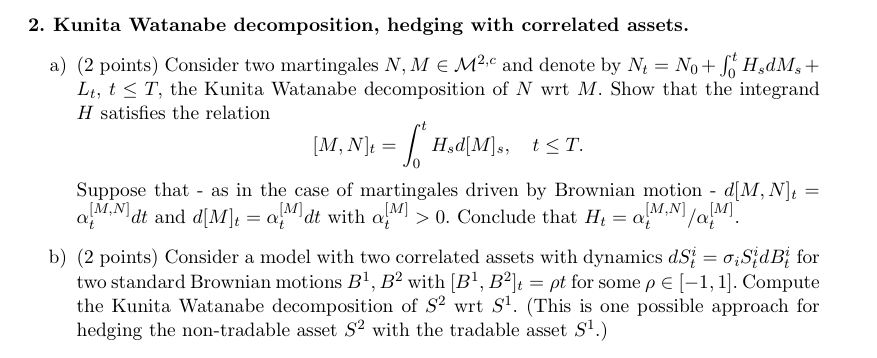
\includegraphics[width=\textwidth]{ex2.png}
\subsection*{a)}
\begin{align*}
	\qcVar{M}{N}_t &= \qcVar{M}{N_0 + \int_0^t H_s dM_s + L_t}_t\\
	&= \qcVar{M}{N_0} + \qcVar{M}{\int_0^t H_s dM_s} + \qcVar{M}{L_t}\\
	&= \qcVar{\int_0^t 1 dM_s}{\int_0^t H_s dM_s}\\
	&= \int_0^t 1 H_s d \qcVar{M_s}{M_s}\\
	&= \int_0^t H_s d \qVar{M_s}
\end{align*}
and \\
\begin{align*}
	\qcVar{M}{N}_t &= \int_0^t H_s d \qVar{M}_s \\
	\Rightarrow	d \qcVar{M}{N}_t &= H_s d \qVar{M}_s \\
	\Rightarrow	\alpha_t^{\qcVar{M}{N}} dt &= H_s \alpha_t^{\qVar{M}} dt \\
	\Rightarrow H_s &= \frac{\alpha_t^{\qcVar{M}{N}}}{\alpha_t^{\qVar{M}}}
\end{align*}

\subsection*{b)} 
We have to calculate the Kunita Watanabe decomposition of $S^2$ wrt. $S^1$. We need to find H and L to find the characterization:
\begin{equation}
S^2 = S_0^2 + \int_0^t H_s d[S^1]_s + L_t
\end{equation}

%From a) we get:
%\begin{align*}
%H_t &= \frac{[S^1, S^2]_t}{[S^1]_t} \\
%	&= \frac{[\int_0^. \sigma_1 S_s^1 d B^1_s, \int_0^. \sigma_2 S_s^2 d B^2_s]_t}{[\int_0^. \sigma_1 S_s^1 d B^1_s]_t} \\
%&=  \frac{\int_0^t \sigma_1 \sigma_2 S_s^1 S_s^2 d [B^1, B^2]_s}{\int_0^t (\sigma_1 S_s^1)^2 d [B^1]_s}\\ 
%&= \frac{\int_0^t \sigma_1 \sigma_2 S_s^1 S_s^2 d \rho s}{\int_0^t (\sigma_1 S_s^1)^2 d s} 
%\end{align*}

From a) we get:
\begin{equation}
H_t = \frac{[S^1, S^2]_t}{[S^1]_t} = \frac{[\int_0^. \sigma_1 S_s^1 d B^1_s, \int_0^. \sigma_2 S_s^2 d B^2_s]_t}{[\int_0^. \sigma_1 S_s^1 d B^1_s]_t} = 
\end{equation}
\begin{equation}
 = \frac{\int_0^t \sigma_1 \sigma_2 S_s^1 S_s^2 d [B^1, B^2]_s}{\int_0^t (\sigma_1 S_s^1)^2 d [B^1]_s} = \frac{\int_0^t \sigma_1 \sigma_2 S_s^1 S_s^2 \rho d s}{\int_0^t (\sigma_1 S_s^1)^2 d s} = \frac{ \rho \sigma_2 S_t^2}{\sigma_1 S_t^1}
\end{equation}

To find $L_t$ we just need to insert $H_t$ into the characterization and we get:
\begin{equation}
S^2_t =  S_0^2 + \int_0^t \frac{ \rho \sigma_2 S_t^2}{\sigma_1 S_t^1} d s + L_t
\end{equation}
\begin{equation}
L_t = S^2_t - S_0^2 - \int_0^t \frac{ \rho \sigma_2 S_s^2}{\sigma_1 S_s^1} d s
\end{equation}
\begin{equation}
L_t = \int_0^t S^2_s d s - \int_0^t \frac{ \rho \sigma_2 S_s^2}{\sigma_1 S_s^1} d s
\end{equation}
\begin{equation}
L_t = \int_0^t S^2_s (1 - \frac{ \rho \sigma_2}{\sigma_1 S_s^1}) d s
\end{equation}

\end{document}
